\hypertarget{dislocation_8cpp}{\section{dislocation.\-cpp \-File \-Reference}
\label{d3/d7f/dislocation_8cpp}\index{dislocation.\-cpp@{dislocation.\-cpp}}
}


\-Definition of constructors and member functions of the \hyperlink{classDislocation}{\-Dislocation} class.  


{\ttfamily \#include \char`\"{}dislocation.\-h\char`\"{}}\*
\-Include dependency graph for dislocation.\-cpp\-:\nopagebreak
\begin{figure}[H]
\begin{center}
\leavevmode
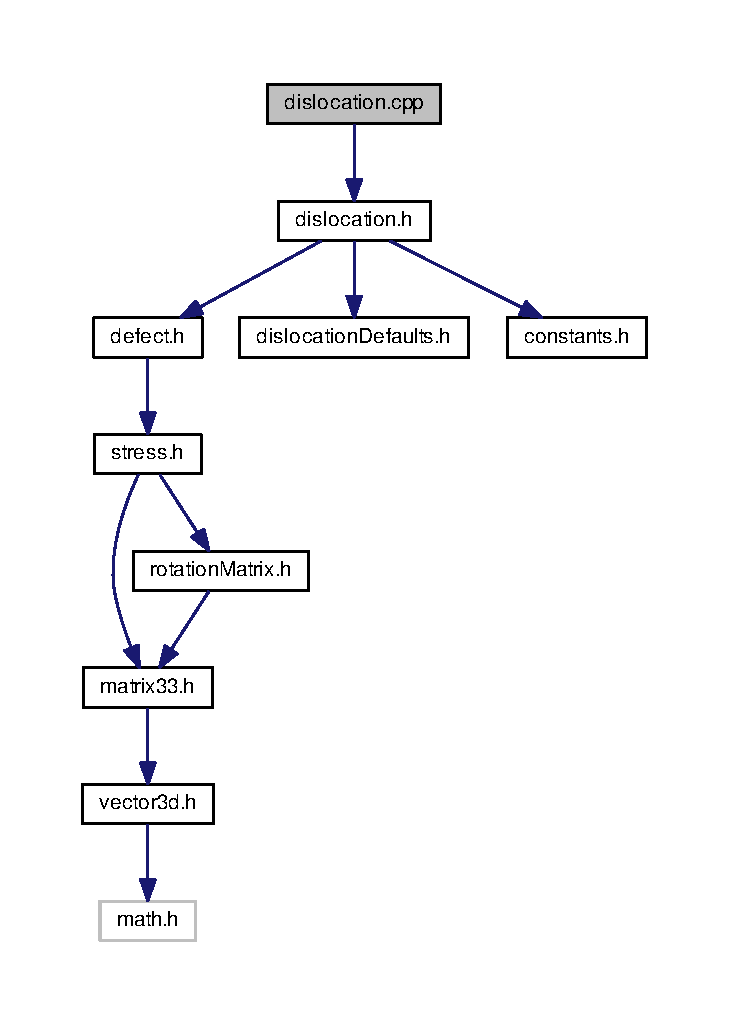
\includegraphics[width=350pt]{d2/d80/dislocation_8cpp__incl}
\end{center}
\end{figure}


\subsection{\-Detailed \-Description}
\-Definition of constructors and member functions of the \hyperlink{classDislocation}{\-Dislocation} class. \begin{DoxyAuthor}{\-Author}
\-Adhish \-Majumdar 
\end{DoxyAuthor}
\begin{DoxyVersion}{\-Version}
1.\-0 
\end{DoxyVersion}
\begin{DoxyDate}{\-Date}
04/06/2013
\end{DoxyDate}
\-This file defines the constructors and member functions of the \hyperlink{classDislocation}{\-Dislocation} class. \-This class inherits from the \hyperlink{classDefect}{\-Defect} class. 

\-Definition in file \hyperlink{dislocation_8cpp_source}{dislocation.\-cpp}.

